\begin{figure}[!t]
\begin{center}

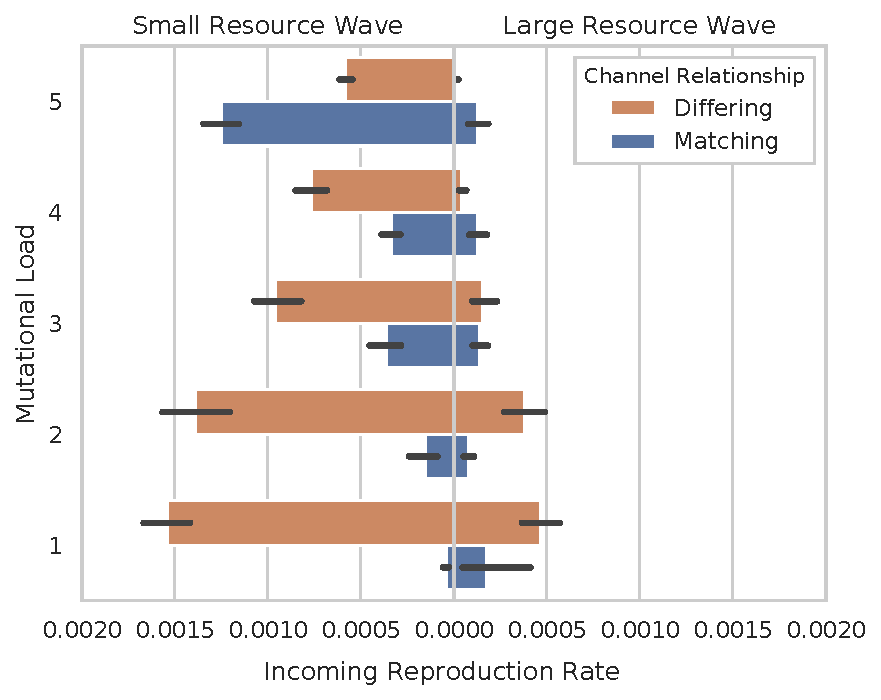
\includegraphics[width=\columnwidth]{title=reproductive_labor+_data_hathash_hash=570375d65c639571+_script_fullcat_hash=7ee0d7e260ffef31+_source_hash=d53f428-clean+ext=}

\caption{
Reproductive cooperation phenotypes by treatment.
Small resource wave treatments are plotted on the left half of the plot, facing leftwards.
Large resource wave treatments are plotted on the right half of the plot, facing rightwards.
Mutational load increases in the upwards direction.
Bar height represents the mean per-update rate at which cells are killed by a neighbor reproducing (e.g., replaced with the neighbor's daughter cell).
Each two-tone pair of bars compares this rate with respect to neighbor cells with matching channels and neighbor cells with differing channels.
Orange bars represent the rate at which cells are killed by different-channel neighbors and blue bars represent the rate at which cells are killed by same-channel neighbors.
Error bars represent 95\% confidence intervals.
The net incoming reproduction rate (e.g., the sum height of bar pairs) differs by treatment because the net resource harvest rate, and therefore net cellular reproduction rate, depends on channel group configuration.
} \label{fig:reproductive_labor}
\end{center}
\end{figure}
